%------------------------------------------------------------------------
% Presentation example for students by Markus Koschi
%
% compile with LaTeX + dvips + ps2pdf or 
% compile with PdfLaTeX after removing all eps figures 

%------------------------------------------------------------------------
\documentclass[shortpres,aspectratio=43]{beamer}
%\documentclass[shortpres,aspectratio=169]{beamer}
\usetheme{CambridgeUS}


\setbeamertemplate{footline}
{
  \leavevmode%
  \hbox{%
  \begin{beamercolorbox}[wd=.333333\paperwidth,ht=2.25ex,dp=1ex,left]{author in head/foot}%
  \hspace*{4ex}\usebeamerfont{author in head/foot}\insertshortauthor%~~\beamer@ifempty{\insertshortinstitute}{}{(\insertshortinstitute)}
  \end{beamercolorbox}%
  \begin{beamercolorbox}[wd=.333333\paperwidth,ht=2.25ex,dp=1ex,center]{title in head/foot}%
    \usebeamerfont{title in head/foot}\insertshorttitle
  \end{beamercolorbox}%
  \begin{beamercolorbox}[wd=.333333\paperwidth,ht=2.25ex,dp=1ex,right]{date in head/foot}%
    %\usebeamerfont{date in head/foot}\insertshortdate{}\hspace*{2em}
    \insertframenumber{} / \inserttotalframenumber\hspace*{2ex}
  \end{beamercolorbox}}%
  \vskip0pt%
}\part{title}
\beamertemplatenavigationsymbolsempty

%color specification-----------------------------------------------------
\definecolor{TUMblue}{RGB}{27, 94, 170}%{rgb}{0.00, 0.40, 0.74}
\definecolor{TUMgray}{rgb}{0.85, 0.85, 0.86}
\definecolor{TUMpantone285C}{rgb}{0.00, 0.45, 0.81}
\definecolor{TUMpantone300C}{RGB}{27, 94, 170} %uncorrected TUMpantone300C
\definecolor{lightblue}{RGB}{213,227,241}%{rgb}{0.7529,0.8118,0.9333}

\setbeamercolor{block title}{fg=white, bg=TUMblue}
\setbeamercolor{block body}{bg=lightblue}
\setbeamertemplate{blocks}[rounded][shadow=true]

%------------------------------------------------------------------------
\setbeamercolor{frametitle}{bg=TUMblue, fg=white}
\setbeamercolor{palette primary}{bg=TUMblue, fg=white}%{fg=TUMblue,bg=TUMgray}
\setbeamercolor{palette secondary}{use=palette primary,bg=TUMblue, fg=white}
\setbeamercolor{palette tertiary}{use=palette primary,fg=white, bg=TUMblue}
\setbeamercolor{palette quaternary}{use=palette primary,fg=white, bg=TUMblue}

\setbeamercolor{title}{bg=TUMblue,fg=white}
\setbeamercolor{item projected}{use=item,fg=black,bg = lightblue}
\setbeamercolor{block title}{fg=black, bg=lightblue}
\setbeamercolor{block body}{bg=white}
\setbeamertemplate{blocks}[rounded][shadow=true]

%------------------------------------------------------------------------
\setbeamertemplate{bibliography item}{\insertbiblabel}
\setbeamercolor{bibliography item}{parent=palette primary}
\setbeamercolor{bibliography entry author}{fg=TUMblue}

%------------------------------------------------------------------------
\usepackage{subfigure}
\usepackage{textpos} % for figure (logo) on slides
\usepackage{psfrag} % for \psfrag in figures
%\usepackage{algorithm,algpseudocode} % for algorithm environment
%\usepackage{booktabs} % for rulers in tables
\usepackage{units} % for units to values
%\usepackage{hyperref}
%\usepackage{graphicx}

%-----------------------------------------------------------------------
\newcommand{\at}{\fontfamily{ptm}\selectfont @}
\newcommand{\ra}[1]{\renewcommand{\arraystretch}{#1}} %to change the row spacing in tables

\newcommand\blfootnote[1]{%
  \begingroup
  \renewcommand\thefootnote{}\footnote{#1}%
  \addtocounter{footnote}{-1}%
  \endgroup
}

%-----------------------------------------------------------------------
\title[Title]{The Title of Your Presentation}

\author[Name]{Your Name}
\institute[TU M\"unchen]{Technical University of Munich}

\date{January~01,~2018}

%---------------------------------------------------------------------
\begin{document}

%% TUM logo
\addtobeamertemplate{frametitle}{}{%
\begin{textblock*}{\textwidth}(.91\textwidth,-0.925cm) % for aspectratio=43

\includegraphics[height=0.65cm]{./figures/TUM_Logo_weiss_e.eps} % for aspectratio=43
%\begin{textblock*}{\textwidth}(.92\textwidth,-0.93cm) % for aspectratio=169
%
\includegraphics[height=0.7cm]{./figures/TUM_Logo_weiss_e.eps} % for aspectratio=169
\end{textblock*}}


\begin{frame}[plain]
    \titlepage
\end{frame}


\section{1. Introduction}

\begin{frame}{Motivation for Set-Based Prediction $[$1$]$}
\blfootnote{\tiny $[$1$]$ M. Althoff and S. Magdici, ``Set-based prediction of traffic participants on arbitrary road networks,'' IEEE Transactions on Intelligent Vehicles, vol. 1, no. 2, pp. 187--202, 2016.}

	\centering	
	\footnotesize
      \psfrag{o}[c][c]{obstacle}						
      \psfrag{c}[c][c]{traffic participant}
      \psfrag{e}[c][c]{ego vehicle}
      \psfrag{f}[c][c]{intended trajectory}      
      \psfrag{w}[r][c]{$t \in [t_0, t_1]$:}
      \psfrag{x}[r][c]{$t \in [t_1, t_2]$:}
      \psfrag{y}[r][c]{$t \in [t_2, t_3]$:}
      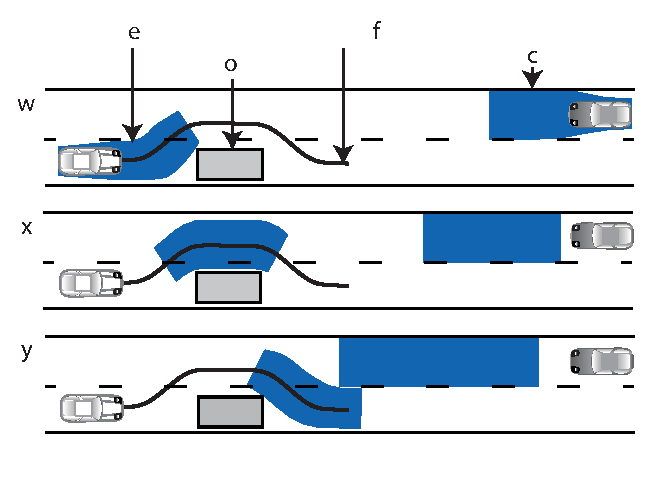
\includegraphics[width=0.8\columnwidth, height=0.74\textheight, keepaspectratio]{./figures/snapshots_blue.eps}
      %\caption{Snapshots of the predicted occupancy of the traffic participant for selected consecutive time intervals.}
\end{frame}


%\begin{frame}{Outline}
%\begin{enumerate}
%\item Item
%\vfill \item Item
%\vfill \item Item
%\vfill \item Item
%\vfill \item Item
%\end{enumerate} 
%\end{frame}


\section{2. Model of the Traffic Participants}

\begin{frame}{SPOT}
SPOT: A tool for set-based prediction of traffic participants $[$2$]$\blfootnote{\tiny $[$2$]$ M. Koschi and M. Althoff, ``SPOT: A tool for set-based prediction of traffic participants,'' in Proc. of the IEEE Intelligent Vehicles Symposium, pp. 1679--1686, 2017.}%\footnote{spot.in.tum.de}
\vspace{1em}

\begin{center}
	{\footnotesize
	\psfrag{a}[r][c]{Obstacle~1}	
	\psfrag{b}[l][c]{Obstacle~2}
	\psfrag{c}[c][c]{Obstacle~3}
	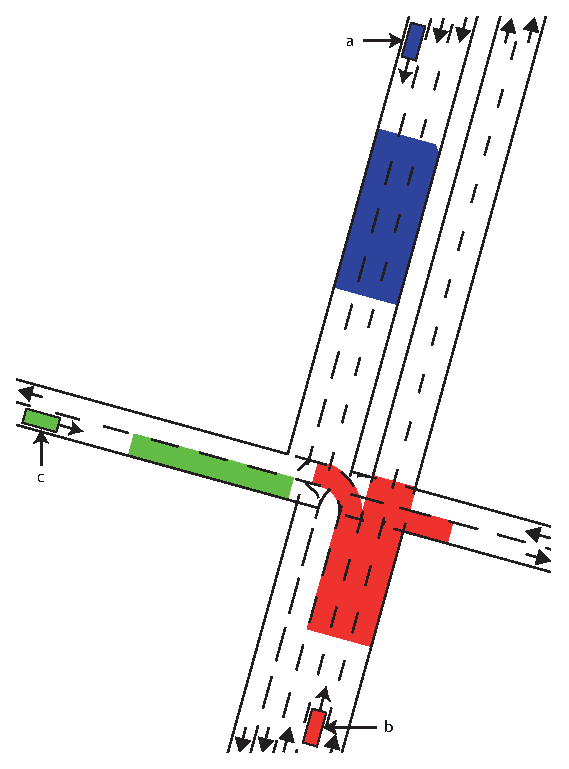
\includegraphics[height=0.5\textheight]{./figures/Scenario_Intersection_Occ_1,5-2,0s_final.eps}
	} \\
	\vspace{1em}
	Initial configuration and $\mathcal{O}(t)$ for $t \in [\unit[1.5]{s}, \unit[2.0]{s}]$
\end{center}

\end{frame}

\section{4. Numerical Examples}



\section{5. Conclusions}
\begin{frame}{Conclusions}

\begin{itemize}
\item Item
\vfill \item  Item
\vfill \item  Item
\end{itemize}

\end{frame}


\end{document}